\newpage
\hypertarget{t2m close}{}
\subsection{Additional \texttt{author} handling}
\genHeader

\begin{itemize}

\item[$\blacktriangleright$] If your project's build succeeded, run \texttt{TGGMain} one more time. Both transformation directions should succeed! Let's examine
the forward direction's output,  \texttt{tree.xmi\_FWD.xmi}, a little closer (Fig.~\ref{eclipse:generatedFwdTrsfm}).

\vspace{0.5cm}

\begin{figure}[htbp]
\begin{center}
  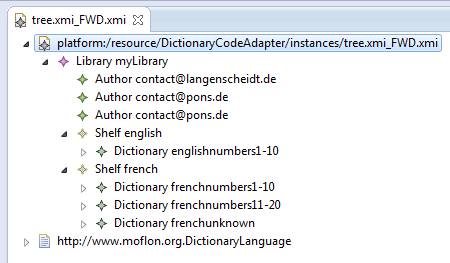
\includegraphics[width=0.7\textwidth]{eclipse_generatedForwardTransformation}
  \caption{completed forward transformation}
  \label{eclipse:generatedFwdTrsfm}
\end{center}
\end{figure}

\vspace{0.5cm}

\item[$\blacktriangleright$] Your output may or may not resemble ours. In fact, there's a 50/50 chance the any of the \texttt{author} nodes were ever created!
Let's run the eMoflon integrator on \texttt{corr\_FWD.xmi} to find out why.\footnote{If you haven't already, read Part IV, Section 6 for details on how this feature
can help you visualise and debug a transformation}

\vspace{0.5cm}

\item[$\blacktriangleright$] Proceed through the transformation until you reach the first match to an author node (Fig.~\ref{eclipse:fwdIntegrator}). Keep an
eye on the small window below -- it states that there are two possible rules that apply to the match!

\begin{figure}[htbp]
\begin{center}
  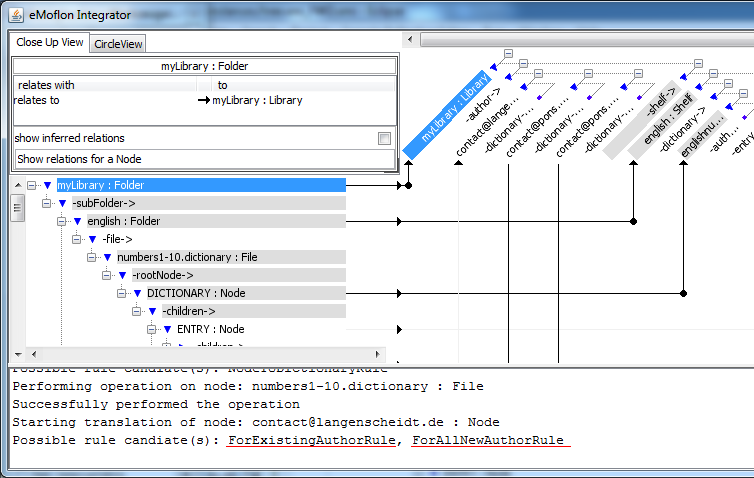
\includegraphics[width=0.8\textwidth]{eclipse_integratorAuthorChoice}
  \caption{completed forward transformation}
  \label{eclipse:fwdIntegrator}
\end{center}
\end{figure}

\clearpage

\item[$\blacktriangleright$] The transformation is presented with, at run-time, a choice between two rules to apply to the matched \texttt{authorNode}.
This setup isn't reliable -- the choice is entirely random, meaning that your output is likely to be different each time you run \texttt{TGGMain}. You therefore
need to force a decision, and there are two ways to do this: at run-time, where users will be able to decide for themselves what they would prefer to use, or at
design-time, where you make the decision a part of the rule.

\end{itemize}

\subsubsection{Option1: Run-time decision}

The advantage with this option is that you leave users with the choice of what they would like to do. Some users don't mind having multiple authors,
while others prefer a miniamlist design. They can easily change their preference here.

\begin{itemize}

\item Create a configuration file for your TGG; First: define \texttt{Author\-Config\-ur\-at\-or}. FIG. put in in the same package as your TGG. Use Eclipse's
auto-completion to help -- don't make errors.

\begin{figure}[htbp]
\begin{center}
  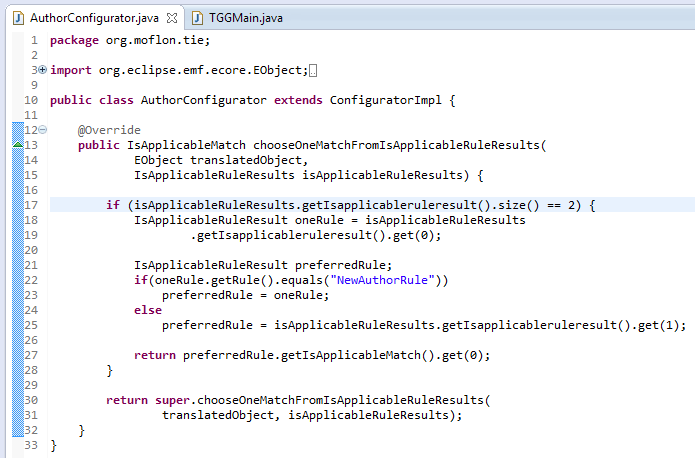
\includegraphics[width=\textwidth]{eclipse_authorConfigurator}
  \caption{comment}
  \label{eclipse:authorConfig}
\end{center}
\end{figure}

\clearpage

\item Second: call it from \texttt{TGGMain}. FIG. Only need it in the forward transformation, so only put it once\ldots

\vspace{0.5cm}

\begin{figure}[htbp]
\begin{center}
  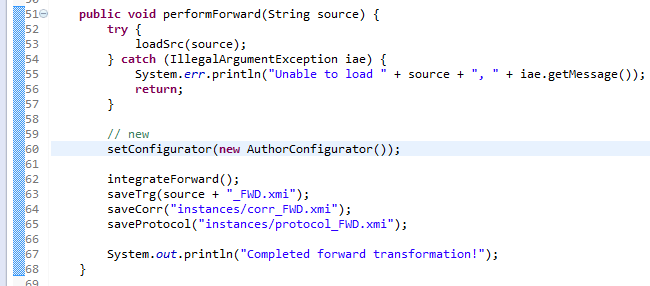
\includegraphics[width=\textwidth]{eclipse_editTGGMain}
  \caption{comment on the edit}
  \label{eclipse:editTGGMain}
\end{center}
\end{figure}

\end{itemize}

\subsubsection{Option 2: Design-time decision}

This deicion is the actual infastracture of the transformation -- users cannot modify this (built-in). Do this by building a NAC to check to see if there is a
contextual author element \emph{with the same email}. You don't want to create this NAC without the attribute constraint or else the transformation will create
only \emph{one} author per library, which is obviously not the case for the \texttt{french} shelf.

\begin{itemize}

\item Depending on your syntax, either update the \texttt{NewAuthorRule} diagram (Visual; Fig.~\ref{ea:existingAuthorNAC}) or the \texttt{ForAllNewAuthor.tgg} 
(Textual; Fig.~\ref{eclipse:existingAuthorNAC}).

\begin{figure}[htbp]
\begin{center}
  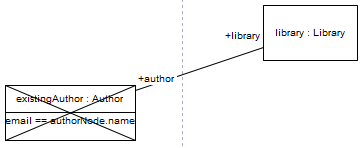
\includegraphics[width=0.7\textwidth]{ea_existingAuthorNAC}
  \caption{comment}
  \label{ea:existingAuthorNAC}
\end{center}
\end{figure}

\begin{figure}[htbp]
\begin{center}
  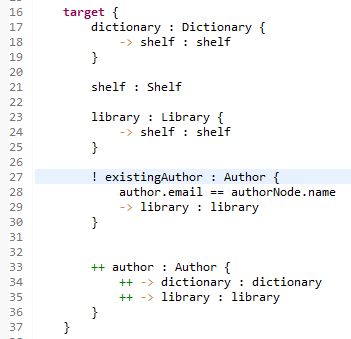
\includegraphics[width=0.7\textwidth]{eclipse_targetNAC}
  \caption{comment}
  \label{eclipse:existingAuthorNAC}
\end{center}
\end{figure}


% Back together, run TGGMain again. 
\newpage

\item[$\blacktriangleright$] Save and rebuild the TGG. Run the transformation a few times, using the integrator to confirm that your preference is executed each
time.

\item[$\blacktriangleright$] Contratulations -- You have now completed a successful Tree-To-Model transformation! The next section begins the backwards
transformation, from Model-To-Text.

\end{itemize}
